%\addtocontents{toc}{\protect\pagebreak}
\chapter{Choix de modèle pour la RLM}
\label{sec:ChoixModeleRLM}

Comme pour la RLS, il est important lors du choix de modèle de s'assurer que les postulats sont bien respectés. Une autre difficulté de la RLM est qu'il faut choisir les variables à inclure dans le modèle parmi toutes celles à notre disposition. Nous abordons ces deux étapes dans ce chapitre.

\section{Vérification des postulats et transformations}

L'analyse des résidus pour la RLM est très similaire à celle des résidus pour la RLS. Nous révisons ici brièvement les notions du chapitre \ref{sec:ChoixModeleRLS}, et introduisons quelques nouvelles procédures.

\subsection{Les résidus}

Comme pour la RLS, le résidu est l'outil de base pour la vérification des postulats. On a déjà vu à la section \ref{sec:distYhatEps} que $\hboeps=\boY-\hY=(\boI_n-\boH)\boY$ et que
\begin{eqnarray*}
	\hboeps \sim \N_n(0, \sigma^2(\boI_n-\boH)).
\end{eqnarray*}

Tout comme pour la RLS, les résidus suivent une loi normale de moyenne $\bm{0}$, mais ne sont pas indépendants et n'ont pas des variances homogènes.

Les résidus standardisés et studentisés sont définis exactement comme pour la RLS:

$$r_i = \dfrac{\hat\varepsilon_i}{\sqrt{\hat\sigma^2(1-h_{ii})}}
\hspace{1cm}
t_i={\hat\varepsilon_i\over \hat{\sigma}_{(i)} \sqrt{1-h_{ii}}}$$


%La plupart des graphiques du Chapitre 2 sont toujours très utiles pour la validation des postulats du modèle et s'interprètent de la m\^eme fa\c{}con qu'auparavant.  Nous traiterons dans les sections suivantes quelques \'etapes de validation d'un modèle de r\'egression lin\'eaire multiple.

\subsection{Vérification de la linéarité}

On peut utiliser les mêmes graphiques que pour la RLS. On doit notamment observer le graphique de  $\hboeps$ \textit{versus} $x_j$ pour toutes les variables explicatives. On pourra alors identifier la ou les variables pour lesquelles la relation avec $Y$ n'est pas linéaire, et corriger le problème par une transformation appropriée.

% Ces graphiques devraient ne montrer aucune tendance, avec les résidus symétriques autour de zéro en ordonnée et une variabilité qui ne varie pas beaucoup en fonction de la valeur de $x_ji$. \vspace{1mm}

Toutefois, \textbf{les graphiques à variable ajoutée} sont mieux adaptés au contexte de la régression multiple pour détecter le manque de linéarité. Un graphique à variable ajoutée est un nuage de points de $\hboeps_{\boY|\boX_{-j}}$ vs $\hboeps_{x_j|\boX_{-j}}$. Ici $\hboeps_{\boY|\boX_{-j}}$ représente le vecteur des
résidus obtenu en régressant $\boY$ sur toutes les variables
exogènes du modèle \textbf{excepté} $x_j$. Il s'agit donc de la partie des $Y_i$ qui n'est pas expliquée par l'ensemble des variables exogènes, sauf la variable d'intérêt.  On veut ensuite savoir si ajouter la variable $x_j$ permet d'expliquer davantage les $Y_i$.  On pourrait tout simplement regarder la relation entre $x_j$ et $\hboeps_{\boY|\boX_{-j}}$, mais puisque $x_j$ peut lui-même être expliqué par les autres variables exogènes, il faut être un peu plus rusé. On utilise donc $\hboeps_{x_j|\boX_{-j}}$, soit le vecteur des résidus de la régression avec $x_j$ comme variable endogène et toutes les variables explicatives sauf $x_j$ comme variables exogènes. On l'obtient en ajustant le modèle suivant:
\begin{equation*}
  x_{ij} = \delta_0+\delta_1x_{i1}+...+\delta{p}x_{ip} +\varepsilon_{i\,[x_j|\boX_{-j}]}.
\end{equation*}
Plus les résidus de cette régression sont grands, plus $x_j$ ajoute de l'information importante au modèle.

Le nuage de points de $\hboeps_{\boY|\boX_{-j}}$ vs $\hboeps_{x_j|\boX_{-j}}$ tombera dans un des trois cas suivants:
\begin{itemize}
\item Si $x_j$ est vraiment une variable qui entre linéairement dans le modèle, \\
 le graphique devrait donner une droite de pente $\beta_j$ passant par l'origine.
\item  Si $x_j$ est \og inutile \fg, \\
le graphique devrait ressembler à un graphique de
résidus ordinaires.
\item  Si $x_j$ est utile mais entre dans le modèle de fa\c{}con non linéaire,\\
 le graphique devrait avoir l'allure d'une courbe plut\^ot que d'une droite.  On pourra donc détecter le manque de linéarité en $x_j$ de la moyenne de $\boY$.
\end{itemize}

\vspace{0.05 in}
Dans certains cas, il est également possible de tester la linéarité d'un modèle à l'aide d'un test de manque d'ajustement. Nous présentons celui-ci à la section \ref{sec:testAjustement}.

\newpage

\subsection{Homogénéité des variances}

On teste l'homogénéité des variances avec le graphique $r_i$ vs $\hat{Y}_i$ comme pour la RLS. S'il y a un problème, on tentera souvent de le régler en transformant la variable endogène.

Notons également qu'il existe un test formel de l'homogénéité des variances, soit le test de \citet{Whi:1980}. La statistique du test de White s'exprime comme suit
$$\chi^2_{\text{White}} = nR^2 \sim \chi^2_{p(p+3)/2}$$
o\`u $R^2$ est le coefficient de détermination ($R^2$) de la régression de $\hat\varepsilon_i^2$ sur toutes les variables explicatives $x_j$, de m\^eme que sur tous les produits croisés entre ces variables, incluant le carré de chacune des variables. On rejette l'hypothèse d'homogénéité des variances au seuil
$\alpha$ lorsque $\chi^2_{\text{White}}>\chi^2_{p(p+3)/2;1-\alpha}$.

\subsection{Normalité des erreurs}

Les mêmes outils que pour la RLS peuvent être utilisés pour tester la normalité des erreurs. Quand le postulat de normalité n'est pas rencontré, il peut \^etre souhaitable  d'utiliser la technique de transformation de Box-Cox (voir section \ref{sec:LaTechniqueDeBoxCox}) pour déterminer la meilleure transformation de la variable endogène.

Il vaut la peine de noter que le test de Shapiro-Wilk est très puissant et que
pour de gros échantillons, il rejettera très souvent la
normalité. Comme les seuils des tests $t$ de Student et $F$ de Fisher ne sont pas
sérieusement affectés si la distribution des résidus est
près de la normalité sans l'atteindre exactement, alors il est
toujours bon d'accompagner le test de normalité d'un diagramme quantile-quantile pour s'assurer que la non-normalité est vraiment sérieuse.

\subsection{Indépendance des erreurs}

On vérifie l'indépendance des erreurs exactement de la même façon que pour la RLS. Si les données sont chronologiques, on peut utiliser un graphique des résidus versus le temps. Sinon, il faut se fier à la description de la collecte de données.

\newpage
\subsection{Test pour manque d'ajustement (lack-of-fit)}
\label{sec:testAjustement}

Ce test permet de vérifier si le modèle proposé s'ajuste bien
aux données. Il constitue un bon complément à l'analyse des
résidus. Toutefois, ce test ne peut être utilisé que lorsque nous avons plusieurs observations dont la (les) variable(s) exogène(s) a (ont) exactement la (les) m\^eme(s) valeur(s).

\begin{exemple}
\label{lof1}
Le tableau \ref{jeuLOF} montre un jeu de données où les observations 2 et 3, 4 et 5 et 7 et 8 ont les m\^emes combinaisons de valeurs pour leurs variables exogènes. Un test de manque d'ajustement est donc possible dans ce cas.

\begin{table}[h!]
\begin{center}
\begin{tabular}{||cccc||cccc||}\hline\hline
Obs & $Y_i$ & $x_{1}$ & $x_{2}$ & Obs & $Y_i$ & $x_{1}$
& $x_{2}$ \\ \hline\hline
 1 &  8.74 & 2 & 1 &&&& \\
 2 & 7.10 & 2 & 0 & 3 & 9.85 & 2 & 0 \\ 4 & 12.1 & 5 & 1 & 5 & 13.1 & 5 & 1 \\
 6 & 14.1 & 5 & 0 &&&& \\
 7 & 18.6 & 8 & 1 & 8 & 15.0 & 8 & 1 \\
 9 & 16.9 & 8 & 0 &&&& \\
\hline\hline
\end{tabular}\end{center}
\caption{Jeu de données pour lequel le test de manque d'ajustement s'applique.}
\label{jeuLOF}
\end{table}
\end{exemple}

Le test de manque d'ajustement se base sur le fait qu'on peut estimer $\sigma^2$ (l'erreur pure) gr\^ace à la variabilité de la variable endogène parmi les observations ayant une m\^eme combinaison de variables exogènes. On peut ainsi séparer notre somme de carrés résiduels en une partie due à l'erreur pure et une partie due au manque d'ajustement du modèle. Mathématiquement, on écrira
$$
{\underbrace{\sum_{k=1}^m\sum_{j=1}^{n_k}(Y_{kj}-\hat{Y}_k)^2}\atop
SC_{res}}={\underbrace{\sum_{k=1}^m\sum_{j=1}^{n_k}(Y_{kj}-\overline{Y}_k)^2}
\atop
SC_{pure}}+{\underbrace{\sum_{k=1}^mn_k(\overline{Y}_k-\hat{Y}_k)^2}
\atop SC_{ajust.}}.$$
o\`u
\begin{itemize}
\item[$\bullet$] $m$ est le nombre de combinaisons distinctes des valeurs des variables exogènes
\item[$\bullet$] $n_k$, le nombre d'observations de la $k^e$ combinaison de variables exogènes
\item[$\bullet$] $Y_{kj}$ la $j^e$ observation de la variable endogène pour la $k^e$ combinaison de variables exogènes
\item[$\bullet$] $\overline{Y}_k=\sum_jY_{kj}/{n_k}$, la valeur moyenne de la variable
endogène pour la $k^e$ combinaison de variables exogènes
\end{itemize}



%La variabilité dans les $Y_i$ peut maintenant \^etre estimée à partir des données ayant les m\^emes combinaisons pour les variables exogènes, et ce m\^eme sans modèle: $$s^2={\sum_{i=1}^m\sum_{j=1}^{n_i}(Y_{ij}-\overline{Y}_i)^2\over\sum_{n_i-1}}.$$


Si le modèle de régression est adéquat, alors $\hat{Y}_k$ sera une bonne estimation de la vraie moyenne de $Y$ pour la $k^e$ combinaison de variables exogènes. Dans ce cas, $\overline{Y}_k$ sera proche de la valeur prédite $\hat{Y}_k$ et la $SC_{ajust.}$ sera petite. On compare $SC_{ajust.}$ à $SC_{pure}$ pour tester l'adéquation du modèle.

On teste donc les hypothèses

$H_0 : E(Y_i) = \beta_0 + \beta_1 x_1 + \ldots \beta_p x_p$ \\
$H_1 : E(Y_i) \ne \beta_0 + \beta_1 x_1 + \ldots \beta_p x_p$

On procède alors à une analyse de variance, résumée au tableau \ref{tab:anovaLOF}.

\begin{table}[h!]
\centering
\begin{tabular}{|c||c|c|c|c|}\hline\
 & dl & SC & CM & $F$  \\ \hline\hline
 Manque &  $m-p'$ & $SC_{ajust.}$ &    $\frac{SC_{ajust.}}{m-p'}$  &     ${SC_{ajust.}/(m-p')\over SC_{pure}/(n-m)}$   \\
 d'ajustement & & & &  \\
 Erreur pure  & $n-m$ & $SC_{pure}$ &   $\frac{SC_{pure}}{n-m}$  & \\
 Erreur totale & $n-p'$ & $SC_{res}$ &    &  \\ \hline
\end{tabular}
\caption{Table d'ANOVA pour un test de manque d'ajustement}
\label{tab:anovaLOF}
\end{table}

On rejette $H_0$ si  $F \ge F_{m-p',n-m,\;1-\alpha}$. On peut également obtenir une valeur de $p$ en comparant notre statistique $F$ à la distribution $F_{m-p',n-m}$.

\vspace{0.05in}
\begin{exemple}
Dans les données de l'exemple \ref{lof1}, on a $m=6$ combinaisons de valeurs différentes pour $(x_{1i},x_{2i})$: $\{ (2,1),(2,0),  (5,1), (5,0), (8,1),(8,0)\}$. \\
On a par exemple $n_2=2$ observations avec $(x_{1i},x_{2i})=(2,0)$, et $\overline{Y}_2=8.475$.\\
On peut calculer les 5 autres moyennes pour obtenir $SC_{pure}$.

On ajuste également le modèle $Y_{ij}=\beta_0+\beta_1x_{1i}+\varepsilon_i$, et on obtient alors $\hat{Y}_1, \ldots, \hat{Y}_6$, ce qui permet de calculer $SC_{res}$ et $SC_{ajust.}$. On trouve:

\begin{center}
\begin{tabular}{||c||c|c|c|c|c||}\hline\hline
  & dl & SC & CM & F & $Pr>F$ \\ \hline\hline
 Manque ajustement &  3 &    1.598029 &    0.53267  &     0.1484   &
 0.9242 \\
 Erreur pure  &  3 &   10.76125 &    3.58708  & & \\
 Erreur totale &  6 &   12.3598 &   2.0599   & & \\ \hline\hline
\end{tabular}
\vspace{5mm}
\end{center}

\vspace{-0.05in}
Il ne semble pas y avoir de problème de manque d'ajustement dans notre exemple. Bien entendu, avec le très petit nombre de données observé, très peu d'hypothèses peuvent \^etre rejetées!
\end{exemple}

\newpage
\section{Importance de la sélection de variables}

Pour la RLM, la vérification des postulats n'est pas le seul élément important dans le choix du modèle. Il faut aussi sélectionner les variables à inclure dans le modèle.

En effet, il se peut que certaines variables dans notre jeu de données de soient pas associées à la variable réponse.
%On verra à la section \ref{sec:inclurevar} qu'il est important d'inclure toute les variables utiles, et seulement celles-ci.
En présence d'un grand nombre de variables exogènes, on court deux dangers: enlever une variable qui est utile pour expliquer la variable endogène, et conserver dans le modèle une variable qui n'est pas utile.

\textbf{Conserver une variable inutile}

Si on conserve trop de variables, on va augmenter inutilement la variance des estimations. Par conséquent, certains effets importants risquent d'être jugés non significatifs.

Plus précisément, supposons que le bon modèle soit:
\begin{eqnarray}
% \nonumber to remove numbering (before each equation)
Y_i &=& \beta_0+\beta_1 x_{1i}+...+\beta_k x_{ki}+ \varepsilon_i.
\label{eq:modelekvar}
\end{eqnarray}
Si on ajoute la variable $x_{k+1}$ et qu'on ajuste le modèle:
\begin{eqnarray}
% \nonumber to remove numbering (before each equation)
\label{eq:modelekplus1var}
  Y_i &=& \beta_0^*+\beta_1^* x_{1i}+...+\beta_k^* x_{ki}+ \beta_{k+1}^* x_{(k+1)i}+ \varepsilon_i
\end{eqnarray}

on obtiendra que $$\var[\hat\beta^*_j] \geq \var[\hat\beta_j],\qquad\text{pour } \;j=1,...,k.$$
De plus, la prévision faite pour $Y$ en un $\bo{x}^*$ donné sera moins précise avec le modèle superflu de l'équation \eqref{eq:modelekplus1var} qu'avec le modèle simple de l'équation \eqref{eq:modelekvar}.

\textbf{Enlever une variable utile}

À l'opposé, si on enlève trop de variables, le modèle sera biaisé. Pour illustrer le biais, prenons par exemple les deux modèles suivants exprimés sous forme matricielle :
\begin{eqnarray}
% \nonumber to remove numbering (before each equation)
  \boY &=& \boX_1\bobeta_1 + \boeps,
  \label{eq:1parametre}
  \end{eqnarray}
  \begin{eqnarray}
  \boY &=& \boX_1\bobeta_1 +\boX_2\bobeta_2 +\boeps,
  \label{eq:2parametres}
\end{eqnarray}
où $\bobeta_1$ comporte $p'=p+1$ paramètres et $\bobeta_2$ inclut $m-p'$ paramètres.

Supposons que le bon modèle soit celui de l'équation \eqref{eq:2parametres} et qu'on choisisse plutôt le modèle de l'équation \eqref{eq:1parametre}, on aura alors
\begin{eqnarray*}
% \nonumber to remove numbering (before each equation)
  \esp[\hbobeta_1] &=& (\boX_1'\boX_1)^{-1}\boX_1'\esp[\boY] \\
  &=&  (\boX_1'\boX_1)^{-1}\boX_1' (\boX_1\bobeta_1 + \boX_2\bobeta_2)\\
  &=& \bobeta_1 + (\boX_1'\boX_1)^{-1}\boX_1'\boX_2 \bobeta_2.
\end{eqnarray*}
On a donc que $\hbobeta_1$ est un estimateur biaisé.

Si l'on s'intéresse plutôt à la prévision au point $\bo{x}^* = \left[\begin{array}{cc}\bo{x}_1^*\\\bo{x}_2^*\end{array}\right]$, le modèle à $p'$ paramètres nous donnerait
\begin{eqnarray*}
% \nonumber to remove numbering (before each equation)
   \hY(\bo{x}_1^{*}) &=& \bo{x}_{1}^{*'} \hbobeta_1 \\
  \esp[\hY(\bo{x}_1^{*})] &=& \bo{x}_{1}^{*'} \esp[\hbobeta_1]  \\
     &=& \bo{x}_{1}^{*'} \{\bobeta_1 + (\boX_1'\boX_1)^{-1}\boX_1'\boX_2 \bobeta_2\}
\end{eqnarray*}
alors que le modèle à $m$ paramètres conduirait à
\begin{eqnarray*}
   \hY(\bo{x}^{*}) &=& \bo{x}_{1}^{*'} \hbobeta_1^* + \bo{x}_{2}^{*'}\hbobeta_2^* \\
  \esp[\hY(\bo{x}^{*})] &=&  \bo{x}_{1}^{*'} \bobeta_1 + \bo{x}_{2}^{*'}\bobeta_2.
\end{eqnarray*}

Le biais dans la prévision serait donc
\begin{eqnarray*}
% \nonumber to remove numbering (before each equation)
   \mbox{biais}[\hY(\bo{x}^{*})]&=&  \esp[\hY(\bo{x}_1^{*})] -\esp[\hY(\bo{x}^{*})]\\
   &=& \bo{x}_{1}^{*'} \{\bobeta_1 + (\boX_1'\boX_1)^{-1}\boX_1'\boX_2 \bobeta_2\} -  \bo{x}_{1}^{*'} \bobeta_1 - \bo{x}_{2}^{*'}\bobeta_2\\
   &=& [{\bo{x}_{1}^{*'}(\boX_1'\boX_1)^{-1}\boX_1'\boX_2}-\bo{x}_{2}^{*'}]\bobeta_2.
\end{eqnarray*}

\textbf{En somme}

En résumé, un trop grand nombre de variables mène à une variance trop grande et un trop petit nombre de variables conduit à une estimation biaisée. Il est donc important de chercher un ensemble de variables permettant d'atteindre un compromis entre ces deux critères. Pour ce faire, on a souvent recours à l'une des techniques de sélection de variables pour choisir un sous-ensemble raisonnable de variables.

\newpage

\section{Critères basés sur l'ajustement du modèle}

Pour sélectionner les bonnes variables dans le modèle, plusieurs techniques sont disponibles. Voyons d'abord quelques critères basés sur l'ajustement du modèle.

\subsection{Coefficient de détermination}

Comme pour la RLS, le coefficient de détermination est défini comme
\begin{equation}\label{R^2}
R^2={SC_{reg}\over SC_{tot}}=1-{SC_{res}\over SC_{tot}}.
\end{equation}

C'est une mesure d'ajustement du modèle facile à calculer et à interpréter, mais il est problématique pour la RLM puisque sa valeur ne peut jamais diminuer si on ajoute une variable dans le modèle, même si celle-ci est inutile.

En effet, si on ajoute un terme à un modèle de régression, $SC_{reg}$ ne peut pas diminuer. Comme $SC_{tot}$ ne dépend pas du modèle, elle reste inchangée. Donc l'ajout d'un terme au modèle se traduit forcément par un $R^2$ plus grand.
%Ainsi, si le ``vrai" modèle générant les données est $Y_i=\beta_0+\beta_1x_{i1}+\varepsilon_i$ et que l'on ajuste ce modèle ainsi que le modèle $Y_i=\beta_0+\beta_1x_{i1}+\beta_2x_{i2}+\varepsilon_i$, il est fort probable que le $R^2$ du second modèle soit supérieur à celui du ``vrai" modèle.
L'ajout de termes superflus réduit en général la précision dans les prévisions, ce qu'on souhaite éviter. Le coefficient de détermination n'est donc pas utile pour la RLM.

\subsection{Coefficient de détermination ajusté}

Il s'agit d'un coefficient de détermination qui pénalise pour l'ajout d'un trop grand nombre de variables. Plus précisément, il est défini comme :
\begin{equation}\label{R^2a}
R^2_{a}=1-{CM_{res}\over CM_{tot}}=1-{SC_{res}/(n-p')\over
SC_{tot}/(n-1)}=1-{(n-1)\hat\sigma^2\over SC_{tot}}.
\end{equation}
Avec $R^2_{a}$, l'ajout d'une variable exogène peut aussi
résulter en une diminution de la statistique.
%Tout comme
%c'était le cas pour $R^2$, la valeur maximale que peut prendre
%$R^2_{ajus}$ est 1.
Comme on peut le voir dans la dernière
égalité de l'équation (\ref{R^2a}), comparer deux
modèles sur la base de leur $R^2_{a}$ est équivalent à
comparer deux modèles sur la base de leur estimation de la
variance des termes d'erreur $\hat\sigma^2$, puisque $SC_{tot}$ et $n$ ne
dépendent pas du modèle choisi.

Notez que peu importe si on utilise $R^2$ ou $R^2_{a}$, on ne peut pas vraiment se fier sur ces statistiques pour comparer des modèles employant des transformations différentes de la variable endogène, ou un modèle avec et un modèle sans ordonnée à l'origine.


\subsection{Critère d'information d'Akaike (AIC)}

%%%%%%%%%%%%%%%%%%%%%%%%%%%%%%%%%%%%%%%%%%%%%%%%%%%%%%%%%%%%%%
% Je crois que les commandes AIC et BIC dans R comptent sigma comme un paramètre du modèle. C'est ce que fait PROC MIXED aussi, car en modélisant la matrice de covariance, on se trouve à ajouter des paramètres au modèle. D'où le p' + 1 au lieu de p' .
% Dans REG et GLMSELECT, le nombre de paramètres est p'.

% Notons que Proc MIXED utilise les formules
% AIC= -2ResLogLike + 2p'
% BIC= -2ResLogLike + ln(n)p'  (que reg et glmselect appellent SBC).
% -2ResLogLike = n ln(SSE/n)+n+nln(2Pi) avec Mixed (ML) et AIC/BIC de R,
% -2ResLogLike = n ln(SSE/n)+n+2        avec GLMSELECT,
% -2ResLogLike = n ln(SSE/n)            avec REG,

% De plus, il faut distinguer entre method=ML et method=REML dans MIXED.

%%%%%%%%%%%%%%%%%%%%%%%%%%%%%%%%%%%%%%%%%%%%%%%%%%%%%%%%%%%%%%

Le critère d'information d'Akaike a été proposé par Hirotsugu Akaike (1974), un
statisticien japonais. Ce critère est assez utilisé dans la pratique et permet d'évaluer
la qualité de l'ajustement d'un modèle. Il est défini de plusieurs façons dans la littérature, mais il est toujours basé sur la log-vraisemblance résiduelle:
\begin{eqnarray*}
-2\ln L(\hbobeta,\hat\sigma^2_{\text{ML}}) & = & \sum_{i=1}^n\frac{(Y_i-\hat Y_i)^2}{\hat\sigma^2_{\text{ML}}}+n\ln(2\pi\hat\sigma^2_{\text{ML}}) \\
& = & n+n\ln(2\pi\hat\sigma^2_{\text{ML}}) \\
& = & n+n\ln(2\pi)+n\ln(SC_{res}/n),
\end{eqnarray*}
car $\hat\sigma^2_{\text{ML}}=\sum_{i=1}^n(Y_i-\hat Y_i)^2/n=SC_{res}/n.$


Les différentes définitions du AIC varient par une constante additive dépendant de $n$. Puisque tous les modèles sont basés sur les mêmes observations (donc le même $n$), on sélectionnera les mêmes variables avec n'importe laquelle de ces versions:

\small
$$\begin{array}{lcc}
\text{Critère}&\text{Procédure SAS }&\text{Fonction R}\\\hline
AIC_1=n\ln(SC_{res}/n)+2p' &\text{REG}& \texttt{ extractAIC, stepAIC}\\
AIC_2=n\ln(SC_{res}/n)+2p'+n+2 &\text{GLMSELECT}& \\
AIC_3=n\ln(SC_{res}/n)+2(p'+1)+n + n\ln(2\pi) && \texttt{ AIC}\\
\end{array}
$$

\normalsize
%$$\mbox{AIC}=-2\ln L(\hbobeta,\sigma^2_{\text{ML}})+2p',$$
%En laissant de côté la constante, $n+n\ln(2\pi)$, la statistique AIC s'obtient alors simplement par l'expression suivante
%$$\mbox{AIC}=n\ln(SC_{res}/n)+2p'.$$
L'AIC prend en compte à la fois la qualité des prédictions du modèle et sa complexité. En
effet, un modèle qui s'ajuste bien sur les observations est associé à une faible valeur de $SC_{res}$
et donc à une faible valeur de $n\ln(SC_{res}/n)$. La complexité du modèle est prise en compte en
ajoutant le double du nombre de paramètres ($2p'$) à cette dernière quantité. Un bon modèle est donc associé à une faible valeur d'AIC.

\subsection{Critère BIC ou SBC}

Le BIC, pour Bayesian Information Criterion, souvent appelé SBC pour Schwarz Bayesian Criterion, est un critère semblable à l'AIC. Il est aussi défini de différentes façons:
%\begin{equation}
%\mbox{BIC}=-2\ln L(\hbobeta,\sigma^2_{\text{ML}})+p'\ln(n)
%\end{equation}


\small
$$\begin{array}{lcc}
\text{Critère}&\text{Procédure SAS }&\text{Fonction R}\\\hline
BIC_1=n\ln(SC_{res}/n)+\ln(n)p' &\text{REG}& \texttt{ extractAIC(...,k=log(n))}\\
                 &\text{GLMSELECT}&  \texttt{ stepAIC(...,k=log(n))}\\
BIC_2=n\ln(SC_{res}/n)+\ln(n)(p'+1)+n+ n\ln(2\pi) && \texttt{ BIC}\\
&& \texttt{ AIC(...,k=log(n))}\\
\end{array}
$$

\normalsize

La seule différence avec l'AIC est que la pénalité pour le nombre de variables grandit avec le nombre d'observations. En général, la pénalité du BIC sera supérieure à celle de l'AIC. Le BIC tend donc à sélectionner des modèles moins complexes que l'AIC.

\section{Méthodes basées sur la puissance de prévision}

Si on se préoccupe beaucoup de la capacité prédictive de notre modèle, on peut utiliser certains critères qui mesurent directement la prévision du modèle plutôt que son ajustement. On pourrait simplement regarder la taille des résidus du modèle puisqu'un meilleur modèle devrait mener à de plus petits résidus. Toutefois, on risque de sous-estimer l'erreur de prévision du modèle puisqu'on triche en quelque sorte en testant la prévision de notre modèle sur les données qui ont été utilisées pour l'estimer. On présente ici quelques alternatives.

\subsection{Utilisation d'un jeu de validation}

Une méthode simple et efficace pour mesurer la capacité de prévision d'un modèle est de séparer notre jeu de données en deux au tout début de l'analyse. Avec la première partie, nommée jeu de données d'entraînement, on estime les paramètres du modèle. On prédit ensuite la valeur de la variable dépendante pour les observations dans la deuxième partie du jeu de données, appelé jeu de validation. On choisit le modèle pour lequel l'erreur résiduelle ($CM_{res}$) dans le jeu de validation est la plus petite.

L'avantage ici est que puisque les observations du jeu de validation n'ont pas été utilisées pour estimer les paramètres du modèle, on a une meilleure estimation de l'erreur de prévision réelle. Toutefois, cela fait moins d'observations pour ajuster le modèle, et donc des estimations moins précises. L'utilisation d'un jeu de validation est donc en général limité aux situations où la taille du jeu de données originale est très grande.

\subsection{La validation croisée}

Si notre jeu de données n'est pas assez grand pour utiliser un jeu de validation, on peut avoir recours à la validation croisée. L'idée est la même que pour le jeu de validation, soit de tester le modèle sur des données qui n'ont pas été utilisées pour l'ajuster, mais ici les données font tour à tour partie du jeu de données d'entraînement et du jeu de données de validation. L'algorithme est le suivant:\\

\begin{enumerate}
\item Diviser les données en $k$ échantillons.
\item Ajuster un modèle sur $k-1$ des échantillons et l'utiliser pour prédire les valeurs dans le dernier échantillon. Calculer l'erreur quadratique moyenne.
\item Répéter $k$ fois l'étape 2  avec un échantillon différent pour le test à chaque fois.
\item Calculer la moyenne des $k$ erreurs quadratiques moyennes.
\end{enumerate}

Cet algorithme permet de bien estimer l'erreur de prévision du modèle pour un choix approprié de $k$, mais peut être assez demandant en temps de calcul.


\subsubsection{Critère PRESS}

Une alternative efficace pour la RLM consiste à utiliser la validation croisée avec $k=n$ échantillons de validation, c'est-à-dire à enlever chacune des observations une à une du jeu d'entraînement.

Soit $\hat{Y}_{i,-i}$ la prévision pour l'observation $i$ obtenue à l'aide d'un modèle de régression estimé sans l'observation $i$. On définit alors le $i^e$ résidu $PRESS$ (pour PREdiction Sum of Squares) comme étant
$$\hat\varepsilon_{i,-i}=Y_i-\hat{Y}_{i,-i}.$$

À première vue, cela semble allonger le temps de calcul, mais il est en fait possible de calculer l'erreur quadratique moyenne de façon analytique dans ce cas.

\begin{theorem}
Le $i^e$ résidu $PRESS$ peut \^etre obtenu à l'aide du
$i^e$ résidu ordinaire et de l'élément en position $i,i$
de la matrice chapeau gr\^ace à la relation
$$\hat\varepsilon_{i,-i}={\hat\varepsilon_i\over1-h_{ii}}.$$
\end{theorem}

Pour comparer des modèles, on peut donc calculer le critère
$$PRESS=\sum_{i=1}^n \hat\varepsilon_{i,-i} =\sum_{i=1}^n(Y_i-\hat{Y}_{i,-i})^2=\sum_{i=1}^n\left({\hat\varepsilon_i\over1-h_{ii}}\right)^2.$$
Le critère $PRESS$ permet de comparer entre eux tous les modèles utilisant la m\^eme transformation pour la variable endogène. \'Evidemment, plus le critère $PRESS$ est faible, plus le modèle prédit bien.

Le critère $PRESS$ peut aussi servir à définir un {\em coefficient de détermination de
prévision} de la manière suivante :
\begin{equation}\label{R^2prev}
R^2_{p}=1-{PRESS\over
SC_{tot}}=1-{\sum_{i=1}^n(Y_i-\hat{Y}_{i,-i})^2\over
\sum_{i=1}^n(Y_i-\overline{Y})^2}.
\end{equation}
Encore une fois, une valeur de $R^2_{p}$ approchant 1 est signe
d'un modèle qui prédit bien, tandis qu'une valeur approchant 0
indique un modèle qui prédit mal.

\begin{remarque}
Il est bon d'examiner également chaque résidu $PRESS$ de fa\c{c}on individuelle. En effet, un modèle précis dont une seule des prévisions est mauvaise pourrait être ind\^ument pénalisé par la somme $PRESS$.
\end{remarque}


\subsection{Le $C_p$ de Mallows}

Il existe également un autre critère de comparaison de modèle basé sur la prévision du modèle, soit le $C_p$ de Mallows. Il est maintenant peu utilisé en pratique, mais nous le décrivons tout de même ici car il s'agit d'un critère classique de sélection de modèle.

\label{sec:LeCpDeMallows}

\subsubsection{Idée}

On a vu précédemment qu'un trop grand nombre de variables cause un problème de variance et qu'un nombre insuffisant de variables induit un problème de biais. Un compromis serait de tenter de minimiser l'erreur quadratique moyenne (EQM) de prévision d'un modèle à $p$ variables lorsque $m$ variables sont disponibles.
\begin{eqnarray*}
  \mbox{EQM}[\hat{Y}(\bo{x^*})] &=& \var[\hat{Y}(\bo{x^*})] + \mbox{biais}^2[\hat{Y}(\bo{x^*})] \\
  &=& \sigma^2\bo{x_1^*}'(\boX_1'\boX_1)^{-1}\bo{x_1^*} + \left\{[{\bo{x_1^*}'(\boX_1'\boX_1)^{-1}\boX_1' \boX_2}-\bo{x_2^*}']\bobeta_2\right\}^2
\end{eqnarray*}
Pour minimiser l'EQM, on fait face à deux difficultés: premièrement,  on ne sait pas quel $\bo{x^*}$ choisir; deuxièmement, l'EQM dépend de $\bobeta_2$, que l'on ne connaît pas. Mallows a donc proposé un autre critère, qui permet de régler le premier problème: on minimise
\begin{eqnarray*}
% \nonumber to remove numbering (before each equation)
  \sum_{i=1}^n \frac{\text{EQM}[\hat{Y}(x_i)]}{\sigma^2}.
\end{eqnarray*}
La division par $\sigma^2$ %ne joue aucun rôle mais
permettra une simplification commode.

\paragraph{Calcul de la portion variance de l'EQM}
\begin{eqnarray*}
% \nonumber to remove numbering (before each equation)
  \sum_{i=1}^n \frac{\var[\hat{Y}(\bo{x}_i)]}{\sigma^2} &=& \sum_{i=1}^n \frac{\bo{x}_{1i}' \var[\hbobeta_1] \bo{x}_{1i}}{\sigma^2} \\
  &=& \sum_{i=1}^n \bo{x}_{1i}' (\boX_1' \boX_1)^{-1} \bo{x}_{1i} \\
  &=& \sum_{i=1}^n \mbox{tr}[\bo{x}_{1i}' (\boX_1'\boX_1)^{-1} \bo{x}_{1i}]  \\
  &=& \sum_{i=1}^n \mbox{tr}[\bo{x}_{1i} \bo{x}_{1i}' (\boX_1'\boX_1)^{-1}] \\
  &=& \mbox{tr}\left[(\sum_{i=1}^n \bo{x}_{1i}\bo{x}_{1i}') (\boX_1' \boX_1)^{-1}\right] \\
  &=& \mbox{tr}\left[(\boX_1'\boX_1)(\boX_1'\boX_1)^{-1}\right] \\
  &=& \mbox{tr}(I_p')=p'
\end{eqnarray*}
Dans le développement ci-dessus, nous avons utilisé le fait que la trace d'un nombre réel est le nombre lui-même et que $\mbox{tr}(AB)=\mbox{tr}(BA).$

\paragraph{Calcul de la portion biais de l'EQM}
La portion biais peut être estimée facilement une fois que l'on réalise que
\begin{eqnarray*}
% \nonumber to remove numbering (before each equation)
  \esp[\hat\sigma_p^2] &=& \sigma^2+\frac{\sum_{i=1}^n \mbox{biais}[\hat{Y}(x_i)]^2}{n-p'}
\end{eqnarray*}
où $\hat\sigma_p^2$ est la variance calculée dans le modèle à $p$ variables. Si $\sigma^2$ était connu, on pourrait estimer $\sum_{i=1}^n \mbox{biais}[\hat{Y}(x_i)]^2$ par $(\hat\sigma_p^2-\sigma^2)(n-p')$. Puisque $\sigma^2$ est inconnu, on l'estime par $\hat{\sigma}^2_{toutes}$, la variance calculée dans le modèle incluant toutes les variables disponibles. Le critère proposé par Mallows est donc le suivant:
\begin{eqnarray*}
% \nonumber to remove numbering (before each equation)
  C_p &=& p' + \frac{(\hat\sigma_p^2-\hat{\sigma}^2_{toutes})(n-p')}{\hat{\sigma^2}_{toutes}}.
\end{eqnarray*}
En pratique, un modèle pour lequel $C_p\approx p'$ (ou
$C_p-p'\approx0$) est un bon modèle. Une fa\c{c}on simple de
choisir un modèle lorsque $k$ variables exogènes sont
disponibles est de calculer le $C_p$ des $2^{k+1}$ modèles
possibles et de prendre celui pour lequel $C_p-p'$ est le plus
faible. Mais en général, on utilise $C_p$ pour cerner un petit
ensemble de modèles raisonnables, et ensuite on utilise d'autres
critères ($PRESS$, $R^2_{a}$, etc.) pour départager ces
modèles. On peut réécrire le $C_p$ de la façon suivante, où $SC_{res}$ est associée au modèle à $p$ variables:
\begin{eqnarray*}
% \nonumber to remove numbering (before each equation)
  C_p &=& \frac{SC_{res}}{\hat{\sigma^2}_{toutes}}+2p'-n
\end{eqnarray*}

%Notez que l'estimateur de $\sigma^2$ utilisé est celui obtenu avec le modèle complet.

%\textcolor{red}{Paragraphe À placer plus tard}
%
%Le $Cp$ de Mallows est le critère à privilégier par rapport aux autres. Dans l'ordre du meilleur au pire critère, on a 1)le Cp, 2) la sélection pas à pas, 3) la méthode d'exclusion, 4) la méthode d'inclusion, 4) le $R^2_{a}$ et 5) le $R^2$. On doit aussi considérer d'autres éléments: 1) l'interprétation, 2) des variables exogènes fortement corrélées entre elles n'apportent pas grand chose au modèle et causent des ennuis (voir le chapitre \ref{sec:Multicolinéarité}) sur la multicolinéarité.


\section{Méthodes algorithmiques}

On a beau avoir des critères pour comparer les modèles 2 à 2, encore faut-il savoir quels modèles comparer. En effet, le nombre de modèles possibles à comparer augmente très rapidement avec le nombre de variables et si $p$ est grand il peut être impossible de tester tous les modèles possibles. Certaines méthodes algorithmiques ont été proposées pour tenter de trouver le meilleur modèle par une série d'optimisations.

%Ces méthodes sont moins recommandées que l'utilisation du $C_p$, mais comme $2^{p+1}$ croit rapidement en fonction de $p$, il peut parfois \^etre impossible de calculer les critères $C_p$, $R^2_{a}$, etc. pour tous les modèles possibles. C'est pour ces raisons, et aussi d\^u à un manque de puissance informatique à l'époque, que des méthodes algorithmiques ont été inventées.

L'utilisation de ces méthodes est toutefois de moins en moins conseillée, pour plusieurs raisons
\begin{itemize}
\item[$\bullet$] Il n'y a aucune garantie de trouver le modèle optimal. Le modèle final est un peu trop adapté à l'échantillon.
\item[$\bullet$] Les procédures sont difficiles à appliquer en présence d'interactions.
\item[$\bullet$] L'inférence à partir du modèle final n'est pas exacte. Les valeurs $p$ sont sous-estimées, car on fait de l'inférence conditionnelle et de multiples tests non indépendants.
\item[$\bullet$] Les données dictent la théorie, alors qu'on voudrait confronter la théorie à des données.
\end{itemize}

Nous décrivons toutefois les 3 méthodes algorithmiques les plus connues.:

\begin{itemize}
  \item \textbf{Méthode d'inclusion}: on entre les variables une à une tant qu'elles sont significatives.
  \item \textbf{Méthode d'exclusion}: on entre toutes les variables, puis on les retire une à une tant qu'il reste des coefficients non significatifs.
  \item \textbf{Méthode pas-à-pas}: On entre une variable, puis à chaque étape on vérifie s'il est justifié d'ajouter ou de retirer une variable.
\end{itemize}

À chaque étape de ces méthodes, il faut choisir un critère objectif qui déterminera s'il est utile d'entrer ou de retirer une variable du modèle. Ce peut être un seuil de test si on procède par statistique de Fisher, ou encore un des critères d'ajustement de modèle vus précédemment.

\newpage
\textbf{Méthode d'inclusion (\textit{forward}) }

\begin{enumerate}
\item Commencer avec $ \; Y_i = \beta_0 + \varepsilon_i$.
\item Identifier la variable $j$ qui améliore le plus le modèle d'après le critère de sélection.
\item Si elle est significative (ou si le critère est amélioré), ajouter cette variable au modèle: $\; Y_i = \beta_0 + \beta_j X_{ij} + \varepsilon_i$
\item Répéter les étapes 2 et 3 jusqu'à qu'aucune variable n'améliore le modèle.
\end{enumerate}


On peut utiliser tout critère de notre choix: $R_a^2$, $PRESS$, $C_p$, $AIC$, $BIC$ ou test $F$ de réduction de modèle (puisqu'on compare des modèles emboîtés).


\textbf{Méthode d'exclusion (\textit{backward})}

%Il s'agit d'une petite modification de la méthode d'inclusion.

\begin{enumerate}
\item Commencer avec le modèle complet (toutes les variables).
\item Identifier, si elle existe, la variable $j$ qui améliore le plus le modèle si on l'enlève (ou qui apporte un gain non significatif une fois les autres prises en compte)
\item Enlever cette variable du modèle.
\item Répéter les étapes 2 et 3 jusqu'à ce qu'aucune variable ne puisse être enlevée pour améliorer le modèle.
\end{enumerate}


\textbf{Méthode pas à pas (\textit{stepwise})}

Cette méthode combine les deux premières.

\begin{enumerate}
\item Commencer avec uniquement l'ordonnée à l'origine: $ \; Y_i = \beta_0 + \varepsilon_i$.
\item Faire un pas avec la méthode d'inclusion.
\item Faire un pas avec la méthode d'exclusion.
\item Répéter les étapes 2 et 3 jusqu'à ce qu'aucune variable ne puisse être enlevée ou ajoutée pour améliorer le modèle.
\end{enumerate}

 On peut spécifier des seuils différents pour l'inclusion et l'exclusion des variables.
\newpage

\begin{exemple}
Prenons un cas avec trois variables et $n=10$ observations pour illustrer les méthodes de sélection de variables dites algorithmiques (inclusion, exclusion et pas à pas). On utilisera ici le test  $F$ de réduction de modèle comme critère d'inclusion et d'exclusion, à l'aide de l'information dans le tableau ci-dessous.

\begin{center}
\begin{tabular}{cc}
  \hline
  % after \\: \hline or \cline{col1-col2} \cline{col3-col4} ...
  Variables du modèle & $SC_{res}$ \\\hline
  \text{aucune} & 30 \\\hline
  $x_1$ & 25 \\
  $x_2$ & 24 \\
  $x_3$ & 20 \\\hline
  $x_1,x_2$ & 6 \\
  $x_1,x_3$ & 15 \\
  $x_2,x_3$ & 12 \\\hline
  $x_1,x_2,x_3$ & 4 \\
  \hline
\end{tabular}
\end{center}

$\bullet$ Si on procède \underline{par inclusion}, avec un seuil d'entrée de $\alpha_E=0,25$:
\begin{enumerate}
  \item On commence avec la variable $x_3$ (la plus importante baisse de $SC_{res}$). On compare le modèle nul et $(x_3)$ avec un test $F$. On obtient $F=\frac{30-20}{20/(10-2)}=4 > F_{0,25;1;8}=1,54$ donc on inclut la variable $x_3$.
  \item On essaie ensuite d'inclure la variable $x_2$ (la plus importante baisse de $SC_{res}$ une fois que $x_3$ est prise en compte). On compare les modèles $(x_3)$ et $(x_2,\,x_3)$. On obtient $F=\frac{20-12}{12/(10-3)}=4,67>F_{0,25;1;7}=1,57$ donc on inclut la variable $x_2$.
  \item Enfin on essaie la variable $x_1$. On compare les modèles $(x_2,\,x_3)$ et $(x_1,\,x_2,\,x_3)$. On obtient $F=\frac{12-4}{4/(10-4)}=12>F_{0,25;1;6}=1,62$ donc on inclut la variable $x_1$.
\end{enumerate}
Le modèle final avec la  méthode d'inclusion est $Y=\beta_0+\beta_1\,x_1+\beta_2\,x_2+\beta_3\,x_3 +\varepsilon$.

$\bullet$ Si on procède \underline{par exclusion}, avec un seuil de sortie de $\alpha_S=0,10$:
\begin{enumerate}
  \item On retire $x_3$ (son retrait cause la plus petite hausse de $SC_{res}$) et on compare les modèles $(x_1,\,x_2)$ et $(x_1,\,x_2,\,x_3)$. On obtient $F=\frac{6-4}{4/(10-4)}=3 < F_{0,10;1;6}=3,78$. On rejette la variable $x_3$ du modèle.
  \item On retire $x_1$ et on compare les modèles $(x_1,\,x_2)$ et $(x_2)$. On obtient $F=\frac{24-6}{6/(10-3)}=21>F_{0,10;1;7}=3,58$. On ne rejette pas la variable $x_1$.
\end{enumerate}

Le modèle final avec la  méthode d'exclusion est $Y=\beta_0+\beta_1\,x_1+\beta_2\,x_2 +\varepsilon$.

\newpage
%On peut faire le même exercice avec la \underline{méthode pas à pas} et le résultat serait, dans ce cas précis, le même que le résultat obtenu par exclusion.
$\bullet$ Si on utilise la \underline{méthode pas à pas} avec $\alpha_E=0,25$ et $\alpha_S=0,10$, on vérifie à chaque étape si une des variables peut entrer, puis si une des variables doit sortir:
    \begin{enumerate}
    \item
        \begin{enumerate}[$\bullet$]
        \item La meilleure candidate pour entrer est la variable $x_3$. Comme dans la méthode d'inclusion, on obtient $F=\frac{30-20}{20/(10-2)}=4>F_{0,25;1;8}=1,54$ donc on inclut la variable $x_3$.
        \item Comme $x_3$ est la seule dans le modèle, c'est la seule candidate pour sortir. Puisque $F=4> F_{0.10,1,8}=3,46$, on la garde dans le modèle.
        \end{enumerate}
         Le modèle à cette étape est $Y=\beta_0+\beta_3\,x_3+\varepsilon$.

    \item
        \begin{enumerate}[$\bullet$]
        \item La meilleure candidate pour entrer est la variable $x_2$. On compare les modèles $(x_3)$ et $(x_2,\,x_3)$. On obtient $F=\frac{20-12}{12/(10-3)}=4,67>F_{0,25;1;7}=1,57$ donc on inclut la variable $x_2$.
        \item On vérifie si $x_2$ et $x_3$ sont toujours pertinentes avec l'arrivée de $x_2$. Comme retirer $x_2$ mène au $SC_{res}$ le plus bas, on compare les modèles $(x_3)$ et $(x_2,\,x_3)$ au seuil de 10\%. Puisque $F=4,67>F_{0,10;1;7}=3,58$ , on garde $x_2$ dans le modèle.
        \end{enumerate}
        Le modèle à cette étape est $Y=\beta_0+\beta_2\,x_2+\beta_3\,x_3+\varepsilon$.

    \item
        \begin{enumerate}[$\bullet$]
        \item Enfin on essaie la variable $x_1$. On compare les modèles $(x_2,\,x_3)$ et $(x_1,\,x_2,\,x_3)$. On obtient $F=\frac{12-4}{4/(10-4)}=12>F_{0,25;1;6}=1,62$ donc on inclut la variable $x_1$.
        \item On vérifie si les 3 variables  sont toujours pertinentes individuellement. Comme retirer $x_3$ mène au $SC_{res}$ le plus bas à deux variables, on compare les modèles $(x_1,\,x_2)$ et $(x_1,\,x_2,\,x_3)$ au seuil de 10\%. $F=\frac{6-4}{4/(10-4)}=3 < F_{0,10;1;6}=3,78$. On rejette la variable $x_3$ du modèle.
        \end{enumerate}

    \end{enumerate}
    Le modèle final avec la méthode pas à pas est $Y=\beta_0+\beta_1\,x_1+\beta_2\,x_2+\varepsilon$.
\end{exemple}

\newpage
\section{Régularisation (ou régression pénalisée)}

La régularisation est une technique statistique très générale qui fait référence au fait d'ajouter une pénalité à un modèle pour pénaliser les modèles trop complexes et éviter le sur-ajustement, particulièrement en présence d'un grand nombre de variables explicatives. La méthode de régularisation qui nous intéresse dans cette section est le LASSO, qui peut être utilisé pour la sélection de variables. Nous présentons d'abord la régression ridge, qui est une méthode de régularisation voisine du LASSO. On introduit un biais dans les estimateurs dans le but de diminuer la variance des prédictions.

\subsection{La régression \og ridge \fg}
\label{sec:ridge}

La régression ridge fut très populaire dans les années 1970-80. Elle consiste à estimer les paramètres de régression en ajoutant une petite constante $k>0$ à la diagonale de la matrice $\boX'\boX$ avant de calculer son inverse. %(On travaille souvent avec des variables centrées pour éliminer l'ordonnée à l'origine.)
On obtient alors
\begin{eqnarray*}
\hbobeta(k) & = & (\boX'\boX+k\boI)^{-1}\boX'\boY  \\
& = & \{(\boX'\boX)\left[\boI+k(\boX'\boX)^{-1}\right]\}^{-1}\boX'\boY  \\
& = & \{\boI+k(\boX'\boX)^{-1}\}^{-1}(\boX'\boX)^{-1}\boX'\boY \\
& = & \{\boI+k(\boX'\boX)^{-1}\}^{-1}\hbobeta.
\end{eqnarray*}

L'estimateur $\hbobeta(k)$ est un estimateur biaisé pour $\beta$, ce qui peut sembler problématique. L'intérêt de l'estimateur réside dans sa variance, qui est donnée par
$$\var[\hbobeta(k)]=(\boX'\boX+k\boI)^{-1}(\boX'\boX)(\boX'\boX+k\boI)^{-1}\sigma^2.$$


Dans certains cas, $\hbobeta(k)$ a une variance largement inférieure à celle de $\hbobeta$, ce qui compense le gain en biais en terme d'erreur quadratique moyenne. On peut d'ailleurs choisir $k$ dans le but de minimiser cette erreur quadratique moyenne.

La régression ridge peut être utile en particulier en présence de multicolinéarité (voir la section \ref{sec:solutionsMulticolinearite}) ou lorsque $p>n$.

Il est dur d'interpréter la valeur de $k$ dans l'estimateur ridge, mais elle est reliée à une contrainte fixée sur la longueur du vecteur $\hbobeta(k)$, i.e. sur $\hbobeta(k)'\hbobeta(k)$. Une formulation équivalente de l'estimateur met en évidence cette interprétation.

\newpage

\textbf{Formulation équivalente}

On peut voir la régression ridge autrement. Elle est équivalente à ajuster une régression linéaire normale mais en ajoutant une pénalité à la somme des carrés. On minimise ainsi
$$ Q_{Ridge}(\beta) = \sum_{i=1}^n (Y_i - (\beta_1x_{i1}+...+\beta_px_{ip}))^2 + \lambda \sum_{j=1}^p \beta_j^2 $$

Nous n'irons pas dans ces détails ici, mais notez qu'on peut écrire le $k$ de la formulation précédente en fonction du $\lambda$ de cette formulation.

En comparaison avec la méthode des moindres carrés originale, cette pénalité force les coefficients estimés à être plus proches de 0 qu'avec le critère des moindres carrés. L'estimateur est toutefois une fonction de $\lambda$, qu'on doit choisir. On choisit en général $\lambda$ à l'aide d'un estimateur du risque de prévision, par exemple la validation croisée.

L'idée d'ajouter une pénalité au critère des moindres carrés pour faire un compromis entre le biais et la variance de l'estimateur est plus générale que la simple régression ridge. En particulier, différentes pénalités peuvent être utilisées pour régulariser. La méthode LASSO utilise une pénalité particulièrement utile pour la sélection de variables.

\subsection{Le LASSO}
\label{sub:lasso}

Le LASSO (\textit{Least Absolute Shrinkage and Selection Operator}) a été proposé par Tibshirani en 1995. On minimise dans ce cas
$$ Q_{Lasso}(\beta) = \sum_{i=1}^n (Y_i - (\beta_1x_{i1}+...+\beta_px_{ip}))^2 + \lambda \sum_{i=1}^p | \beta_j | $$

Notez que la seule différence avec la régression ridge est qu'on somme les valeurs absolues des coefficients estimés dans la pénalité, et non les carrés de ces mêmes coefficients.  L'avantage du LASSO est que cette pénalité ne fait pas que biaiser les estimations vers 0, elle force certains coefficients à valoir exactement 0. On a donc directement une sélection de modèle! La figure \ref{fig:lasso} illustre pourquoi c'est le cas.

\begin{figure}[h!]
\centering
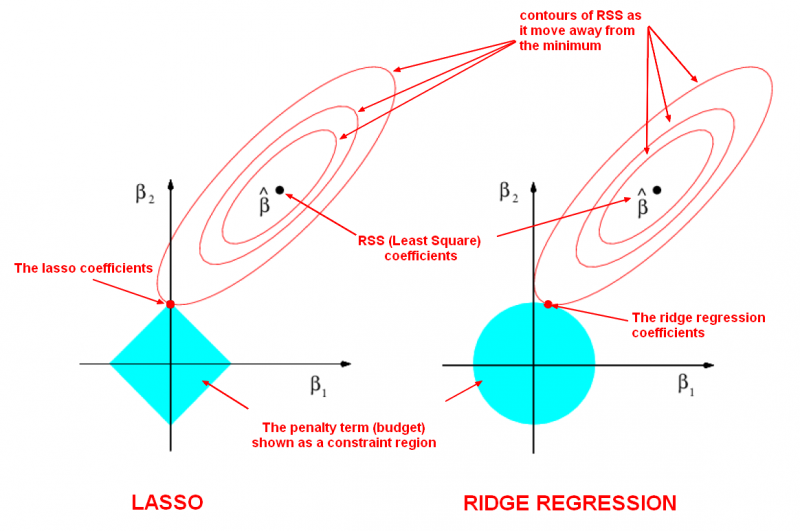
\includegraphics[scale=0.5]{Chap8-ChoixModeleRLM/Figures/lasso_vs_ridge_regression}
\caption[Illustration de la différence entre le LASSO et la régression ridge.]{Illustration de la différence entre le LASSO et la régression ridge. \\{\footnotesize Source : \url{http://gerardnico.com/wiki/data_mining/lasso}}}
\label{fig:lasso}
\end{figure}

\newpage

Tel qu'indiqué plus haut, il faut choisir le paramètre $\lambda$ pour obtenir une estimation avec le LASSO. Celui-ci est généralement choisi pour minimiser l'erreur de prévision, telle qu'estimée par une méthode comme la validation croisée.

Notons que sous certaines hypothèses, on peut montrer que le LASSO identifie correctement les coefficients qui ne valent pas 0 avec une grande probabilité. Toutefois, les estimateurs sont en général biaisés vers 0, et pas nécessairement convergents. En pratique, on utilise donc parfois le LASSO pour faire une sélection de variables, et on estime ensuite les coefficients avec la méthode des moindres carrés sans pénalité.

Enfin, un autre avantage de la régression LASSO est qu'elle permet d'ajuster un modèle dans le cas où le nombre de paramètres à estimer $p'$ est supérieur au nombre d'observations $n$.

\newpage

\section{Le cas des variables catégoriques et interactions}

Dans le cas de modèles de régression contenant des variables catégoriques et des interactions, il faut être un peu plus prudent dans la sélection de modèle.

\subsection{Sélection de modèle avec variables catégoriques}

La sélection se fait comme à l'habitude en présence de variables dichotomiques.

Avec des variables polytomiques, la règle utilisée en sélection de modèle, quel que soit le
critère de sélection, est que les $\beta$ correspondant à une m\^eme variable polytomique soient ou bien tous exclus du modèle, ou bien tous inclus dans le modèle. On peut aussi décider de fusionner certaines catégories de la variable polytomique si c'est suggéré par la forme du modèle sélectionné.

\begin{exemple}
Considérons de nouveau l'exemple \ref{eg:lot}. Si un critère de sélection indique que le meilleur modèle est $Y_i=\beta_0+\beta_{11}x_{11i}+\beta_{13}x_{13i}+\varepsilon_i$, alors on ajoutera $\beta_{12}x_{12i}$ à ce modèle car $\beta_{11}$, $\beta_{12}$ et $\beta_{13}$ sont tous reliés à la variable \og lot \fg et doivent donc ou tous \^etre inclus dans le modèle, ou tous \^etre exclus du modèle, et comme au moins un
de ces $\beta$ semble important, nous les incluons tous. On pourrait aussi décider de fusionner les lots 1 et 2 pour créer une nouvelle variable à trois catégories.
\end{exemple}




\subsection{Sélection de modèle en présence d'interactions}

Si une interaction entre plusieurs variables exogènes est incluse
dans un modèle, on laisse en général les effets plus simples
correspondants dans le modèle. Ceci facilitera l'interprétation des différents coefficients du modèle.

\begin{exemple}
Supposons que le modèle complet est
$$Y=\beta_0+\beta_1x_{1}+\beta_2x_{2}+\beta_3x_{3}+
\beta_{12}x_{1}x_{2}+\beta_{13}x_{1}x_{3}+\beta_{23}x_{2}x_{3}+\varepsilon,$$
mais que les procédures de sélection de variables indiquent que seulement les coefficients $\beta_1$ et $\beta_{23}$
semblent importants.
Nous utiliserions alors le modèle
%$$Y_i=\beta_0+\beta_1x_{1i}+\beta_2x_{2i}+\beta_3x_{3i}+\beta_{23}x_{2i}x_{3i}+\varepsilon_i$$
$$Y=\beta_0+\beta_1x_{1}+\beta_2x_{2}+\beta_3x_{3}+\beta_{23}x_{2}x_{3}+\varepsilon$$
car avec la présence de $\beta_{23}$ dans le modèle, il est
recommandé d'y inclure $\beta_2$ et $\beta_3$.
\end{exemple} 